\documentclass{article}
\usepackage[paper=a4paper]{geometry}
\usepackage{authblk}
\usepackage{xspace}
\usepackage{graphicx}
\usepackage{url}
\usepackage{paralist}

\begin{document}
\title{Using {\LaTeX} in Schools: Simplifying Inclusive STEM Education}

\author[1]{Michael Schäffler, Barbara Henn}
% \email{zainab@kebab-ca.se}
\affil[1]{
  SBBZ Ilvesheim, Germany
}

\author[2]{Volker Sorge}
% \email{austind@gvsu.edu}
\affil[2]{%
  MathJax Consortium
}

\author[3]{Dorine in't Veld}
% \email{v.sorge@bham.ac.uk}
\affil[3]{
  Dedicon, The Netherlands
}

\date{}
\maketitle


\section{Introduction}\label{sec:intro}

We report on experience of the use of {\LaTeX} in Schools to teach mathematics to
blind and visually impaired children. For the last 20 years the German education
has phased out the use of sophisticated mathematical Braille notations and
replace it by teaching children from year one {\LaTeX} (or {\LaTeX}-like) notation in
mathematics. This notation made tactile by translating it into 8-dot Euro
Braille thus removing the use of indicators and the need express single
characters with multiple Braille cells. The aim was to reduce the learning curve
for students as well as to improve their abilities to author and communicate
mathematics with peers and teachers that are not trained in Braille, which is
paramount for inclusive education.

We present how this approach can technically supported via web technology that
can not only render {\LaTeX}, but also provide 8 dot Braille output for expressions
as well as compute meaningful {\LaTeX} commands for sub-expression and support for
direct copying from web sites.

Finally, we will discuss our initial steps to transfer this model to other
education systems, namely the Dutch system, where the current approach is
ambivalent, in that there exists an AsciiMath-like linearized math notation for
teaching to BVI students, while tactile math textbooks use an outdated Braille
notation, that is effectively no longer used in teaching.  As a result students
are actively discouraged from studying mathematics.

\section{{\LaTeX} in Education for the Blind}\label{sec:latex-in-schools}

The choice of mathematical notation in education for blind and visually impaired
(BVI) students vary widely throughout the world. While there exist many national
and regional variations in regular mathematical notation, these differences are
particularly strong for primary and secondary education and become less
pronounced in advanced mathematics and higher education. For BVI learners
however this is generally not the case.

Traditionally, mathematics is presented in tactile format on the basis of highly
specialized Braille notations increases in complexity for more advanced
mathematical notation and more unconventional symbols. In particular, in
traditional 6-dot Braille systems symbols have to be embellished with a plethora
of indicators (e.g., for numbers, capital letter, fonts) and modifiers (for
accents, positioning etc.). For a comparison of notational systems
see~\cite{van2022towards}.

This approach has a number of drawbacks: 
\begin{inparaenum}
\item The learning curve for mathematics, already steep for sighted students,
  becomes even steeper for BVI students.
\item Students can not easily communicate their Braille math with their sighted
  peers or teachers not trained in the formalism, which is an obstacle for
  inclusive education.
\item Math braille notation is usually easier to read but less suitable for
  writing mathematics. This is particularly compounded by the use of computers
  even with Braille input devices.
\item Many traditional math Braille notations have a 2D variant for complex
  elements like nested fractions or matrices, which are difficult to display on
  a computer Braille display.
\item Different Math Braille notations are generally not compatible and often
  even mutually intelligible. Not only have different countries different
  notations, but even the same language has different Math Braille dialects,
  e.g., in English there exist Namath and EBB as well as formerly British Math
  Braille etc.
\end{inparaenum}

As consequence more than 20 years ago Germany has chosen a different path for
specialist education for BVI students. Instead of continuing to teach the local
mathematical Braille notation (Marburg System) based on 6-dot Braille and instead
adopting uniform {\LaTeX} notation for writing and transcribing it into 8-dot
Euro Braille. This has the advantage that 
\begin{inparaenum}
\item there is no need for indicators and
  modifiers as every single ASCII character can be translated into its equivalent
  Euro Braille cell, i.e., every single character of the {\LaTeX} code corresponds
  to exactly one Braille cell.
\item {\LaTeX} is a linear notation and as such can be easily input with
  keyboard and output on the Braille display.
\item The notation helps students to communicate their mathematics with their
  teachers and sighted peers. Simple expressions are easy to understand even for
  those not yet exposed to {\LaTeX} syntax. And if that fails it can be visually
  rendered for easier reading.
\item {\LaTeX} is the lingua franca among mathematicians and as such
  internationally understood notation. Thus students going on to higher
  education are already equipped with the most important tool to communicate
  mathematics with their professors.
\end{inparaenum}


\section{{\LaTeX} to Braille}\label{sec:latex-to-braille}

Obviously in early primary education very little {\LaTeX} is actually
needed. And even then main goal is use as much as possible symbols that are
available on the keyboard. For example, asterisk \texttt{*} is used instead of
\verb+\cdot+ for multiplication and simple fractions are written in beveled
notation e.g., $\frac{1}{2}$ would be written as \texttt{1/2} instead of
\verb+\frac{1}{2}+. Other conventions are adopted for easier reading, such as
avoiding curly braces as much as possible, and inserting spaces before operators
and relation symbols. For example, ${ n! = n*(n-1)! }$ is written by convention
as \verb+n! =n *(n -1)!+

In addition, certain command abbreviations are introduced, primarily with the
goal of reducing spatial requirements on the Braille display. E.g., writing
\verb+\f+ instead of \verb+\frac+, or \verb+\ol+ instead of \verb+\overline+
. Also commands can be replaced by meaningful symbol combinations, such as
\verb+\le+ being replaced by \verb+<=+  (see also \url{https://augenbit.de/}).

Initial online support for working with {\LaTeX} and Euro Braille was developed
at the SBBZ Ilvesheim as an extension of the MathJax v2.7~\cite{MathJax16-w4a}
library. The extension allowed to expose the {\LaTeX} sources in the web page
from which the MathJax would compute the visual rendering as textual underlay
for the expression. This allowed easy selection and copying and pasting into a
text editor or word processor from which the expression could be automatically
translated into 8-dot Braille by a correctly configured screen reader. While
this technique was sufficient for students to work with, in particular during
the Covid pandemic, it had the drawback that, while some cleanup on the {\LaTeX}
source could be done, the expression would usually not follow all the rules
described above.

In MathJax version 4~\cite{mathjax20siam} we will support these features
natively, in particular, copying and Euro Braille translation and rewriting
{\LaTeX} sources into the required format. Figure~\ref{fig:eurobraille} shows
the Braille translation for the commands describing the quadratic equation:

\[
\verb+x = \frac{-b \pm \sqrt{b^2-4ac}}{2a}+
\]

\begin{figure}
  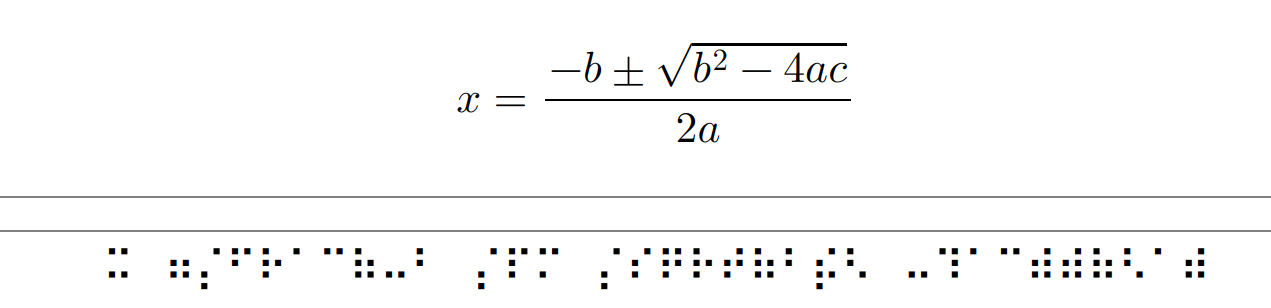
\includegraphics[width=.9\textwidth]{quadratic.png}
  \caption{Translation of the quadratic equation into 8-dot Euro Braille}
  \label{fig:eurobraille}
\end{figure}

As an additional feature MathJax v4 exposes correct {\LaTeX} sub expressions for
parts of formulas that can be interactively explored. While this sounds
straightforward, these sub expressions are non-trivial to compute. Firstly,
{\LaTeX} is a touring complete language, which requires a recursive stack
automaton for parsing and thus partial expressions are not as readily available
as in a simple LR-parser. Secondly, the exploration is based on a semantic model
that is computed using Speech Rule Engine~\cite{sre}, which produces a
canonical purely semantic representation of the math expression regardless of
the incoming syntax, i.e., {\LaTeX}, MathML, or AsciiMath..

\begin{figure}
  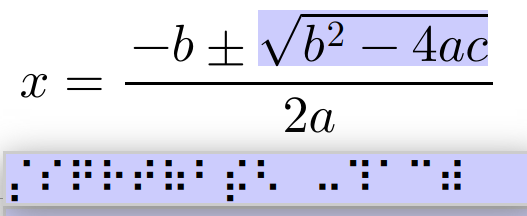
\includegraphics[width=.6\textwidth]{quadratic-square.png}
  \caption{Translation of the quadratic equation into 8-dot Euro Braille}
  \label{fig:subbraille}
\end{figure}

Figure~\ref{fig:subbraille} shows the Braille for the square root sub expression
in the quadratic formula.\footnote{Additional examples of the technique can be found
here: \url{https://mathjax.github.io/MathJax-demos-web/euro-braille/}} Note that
there are nevertheless limits to the {\LaTeX} sub expression MathJax can
produce. For example, AMS matrix environments like \texttt{pmatrix},
\texttt{bmatrix}, or \texttt{vmatrix} implicitly generate fences, that are
rendered. However, at the moment the parsing algorithm cannot produce
corresponding {\LaTeX} output.

\section{Math Notation in the Netherlands}\label{sec:math-netherlands}

While similar approaches to math braille notation have been taken in other
European countries using established mathematical syntax notations (e.g.,
{\LaTeX} in Slovenia and AsciiMath in Sweden), other countries have pursued a
different approach.

We will examine the situation in The Netherlands. Over twenty years ago in The
Netherlands math had become practically inaccessible, the primary problem being
the lack of a braille math code. Consequently, a linear notation was developed
and introduced by Dedicon\footnote{\url{http://braille.dedicon.nl/wiskunde}}, which eases
math communication in particular in inclusive education, but did not follow any
pre-existing standards.

One of the notation's strong points is that it remains consistent
notwithstanding in what application it is used. It can be converted from
Microsoft Word or HTML to plain text or Markdown without a problem. That is
because the notation only uses characters that can be typed with a qwerty
keyboard. It can be used for direct communication without requiring additional
assistive or conversion software. Likewise, its translation into Braille is
straightforward in particular when using 8-dot Euro Braille.

The weaknesses are that the notation initially only covered primary and
secondary education, not higher education. And while it was good for writing, it
was too ambiguous for more complex expressions, mainly due to its use of spaces
for delineation. For example, there is a rule that spaces terminate superscript
and subscript text, which is usually very convenient but can go wrong when
combining the two: Consider \verb+x_2 ^2+ versus \verb+x_2^2+, where the former
is $x_2^2$, while the latter is represents $x_{2^2}$. Note that the space the
$2$ and the caret symbol makes the difference, which can lead to easy mistakes.
The main issue is the lack of clear notation that defines argument boundaries,
which is particularly concerning with more complex expressions containing
fractions, roots, vectors etc.  As a consequence, automatic conversion is
difficult and there currently exists no implementation of a renderer that can
visualize expressions.

As an initial step we therefore aimed at moving from the Dedicon notation to
AsciiMath. However, we are now in the process of exploring the possibility to
follow the German model and introducing {\LaTeX} as the basic language of math
exchange.  One major obstacle that we need to overcome is that our current
production pipeline for electronic documents, translates printed math material
into MathML rather than into {\LaTeX}, which would be more future proof and more
helpful for the students in the next generations.

% \clearpage
\bibliographystyle{plain}
\bibliography{bibs}


\end{document}


%%% Local Variables:
%%% mode: latex
%%% TeX-master: t
%%% End:
